\clearpage
\section{The effect of query plan cache}
Every query requires a query plan before it is actually executed. Whenever a query is run for the first time in MongoDB, a query plan is generated for the query. This query plan is cached with the shape of the query. In this way, when the queries with the same shape are run again, MongoDB reuses the cached query plan instead of creating a new one. 

Recall that query shape is essentially a query’s match expression, projection and sort with the values taken out. Therefore, all queries in the previous experiments have exactly the same query shape despite different query range. As a result, after the first query is executed, all other query statements will use its cached query plan. 

In this experiment, we aim at exploring the effect of query plan cache. Therefore, we simulated three cases where different query plan was cached first: 
\begin{enumerate}
    \item Plan A cached: An index scan on field A was cached first.
    \item Plan B cached: An index scan on field B was cached first.
    \item Plan C cached: A collection scan was cached first.
\end{enumerate}
As a result, all other queries will reuse the query plan of the first query that has been executed. We compared the execution time of the cached plan with that of the optimal plan (i.e. the query plan that has the shortest execution time). An impact factor is calculated based on averaging over plans from different selectivity.

\subsection{Without covering index}
\begin{figure}[htb]
    \centering
    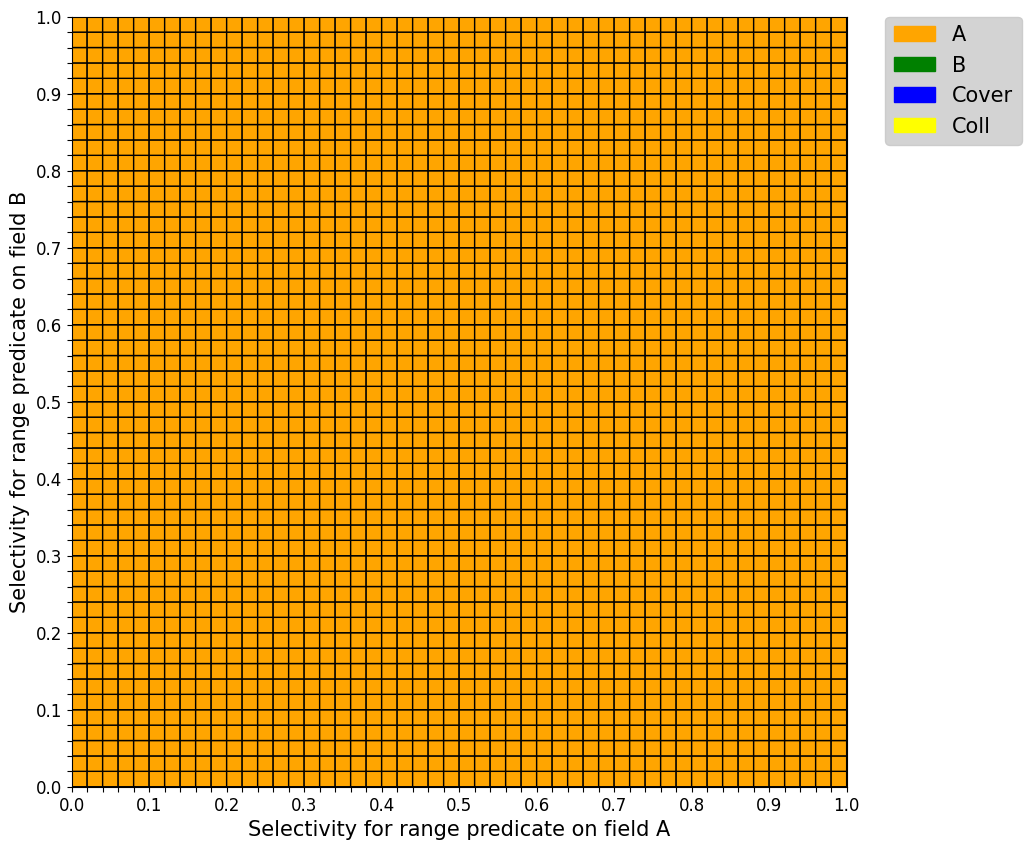
\includegraphics[width=0.6\linewidth]{images/results-without-covering-index/mongo-original/plan_a_cached_mongo_choice.png}
    \caption{Plan A cached: MongoDB's chosen plans}
    \label{fig:a-cached-v0}
\end{figure}


\begin{figure}[htb]
    \centering
    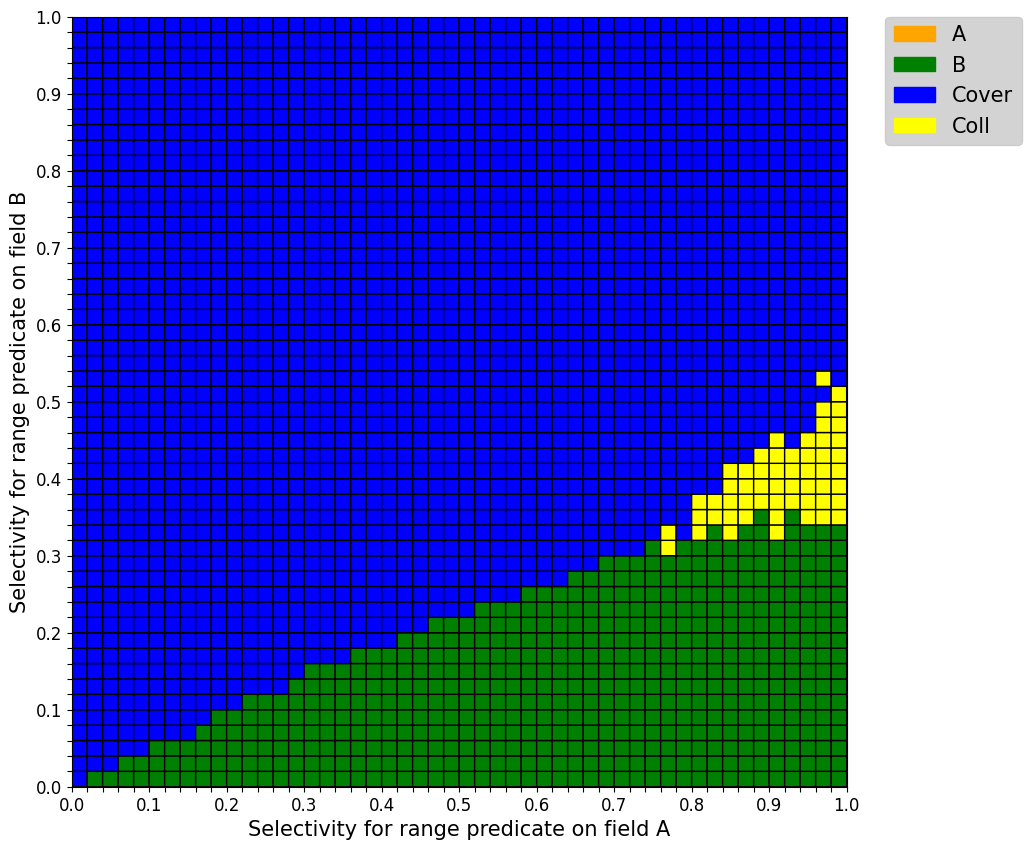
\includegraphics[width=0.6\linewidth]{images/results-without-covering-index/mongo-original/plan_a_cached_practical_winner.png}
    \caption{Plan A cached: the optimal query plans}
    \label{fig:a-cached-optimal-v0}
\end{figure}


\begin{figure}[htb]
    \centering
    \includegraphics[width=0.5\linewidth]{images/results-without-covering-index/mongo-original/plan_a_cached_summary_accuracy=24.92_overall_percentage_change=251.81.png}
    \caption{Plan A cached: MongoDB's chosen plans, accuracy = 24.92\%, impact factor = 251.81\%}
    \label{fig:a-cached-impact-v0}
\end{figure}


\begin{figure}[htb]
    \centering
    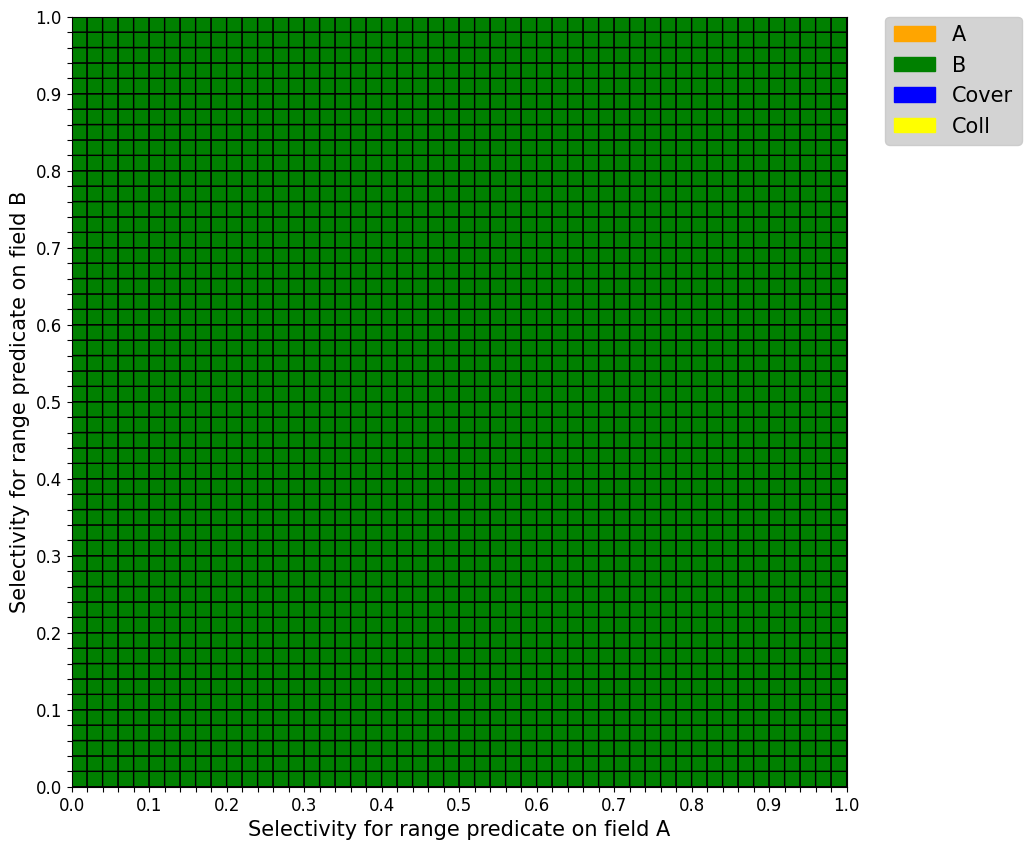
\includegraphics[width=0.6\linewidth]{images/results-without-covering-index/mongo-original/plan_b_cached_mongo_choice.png}
    \caption{Plan B cached: MongoDB's chosen plans}
    \label{fig:b-cached-v0}
\end{figure}


\begin{figure}[htb]
    \centering
    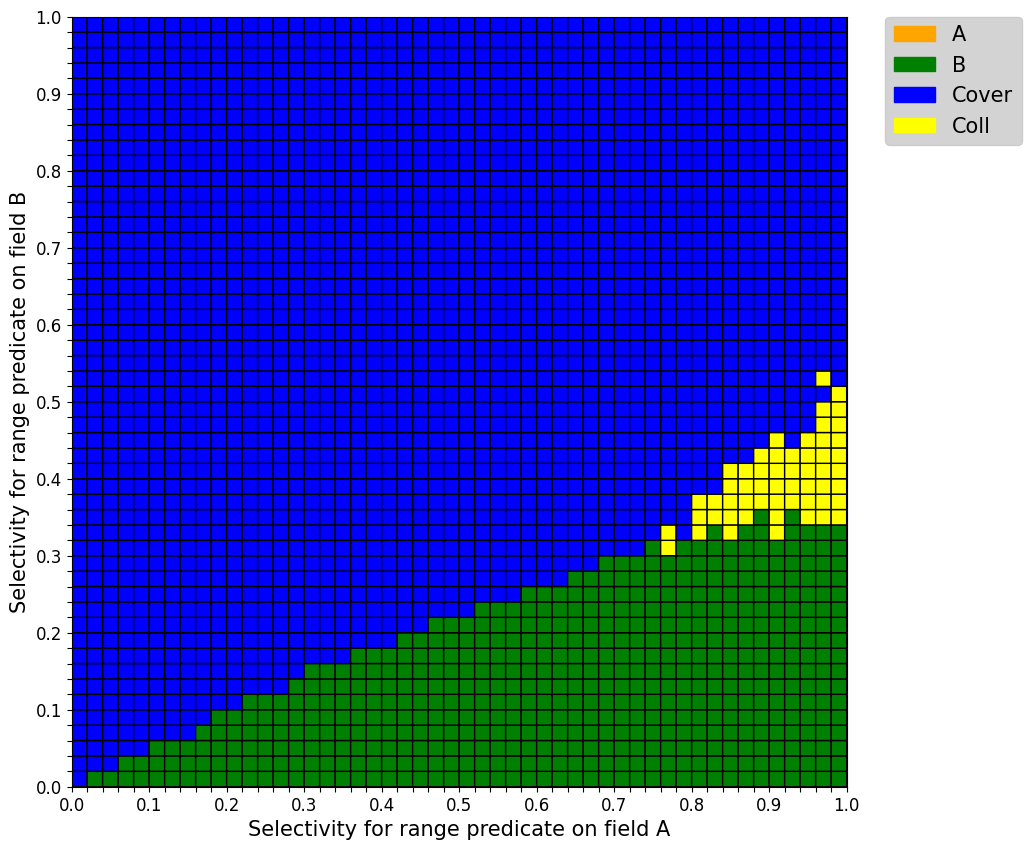
\includegraphics[width=0.6\linewidth]{images/results-without-covering-index/mongo-original/plan_b_cached_practical_winner.png}
    \caption{Plan B cached: the optimal query plans}
    \label{fig:b-cached-optimal-v0}
\end{figure}


\begin{figure}[htb]
    \centering
    \includegraphics[width=0.5\linewidth]{images/results-without-covering-index/mongo-original/plan_b_cached_summary_accuracy=27.60_overall_percentage_change=222.32.png}
    \caption{Plan B cached: MongoDB's chosen plans, accuracy = 27.60\%, impact factor = 222.32\%}
    \label{fig:b-cached-impact-v0}
\end{figure}


\begin{figure}[htb]
    \centering
    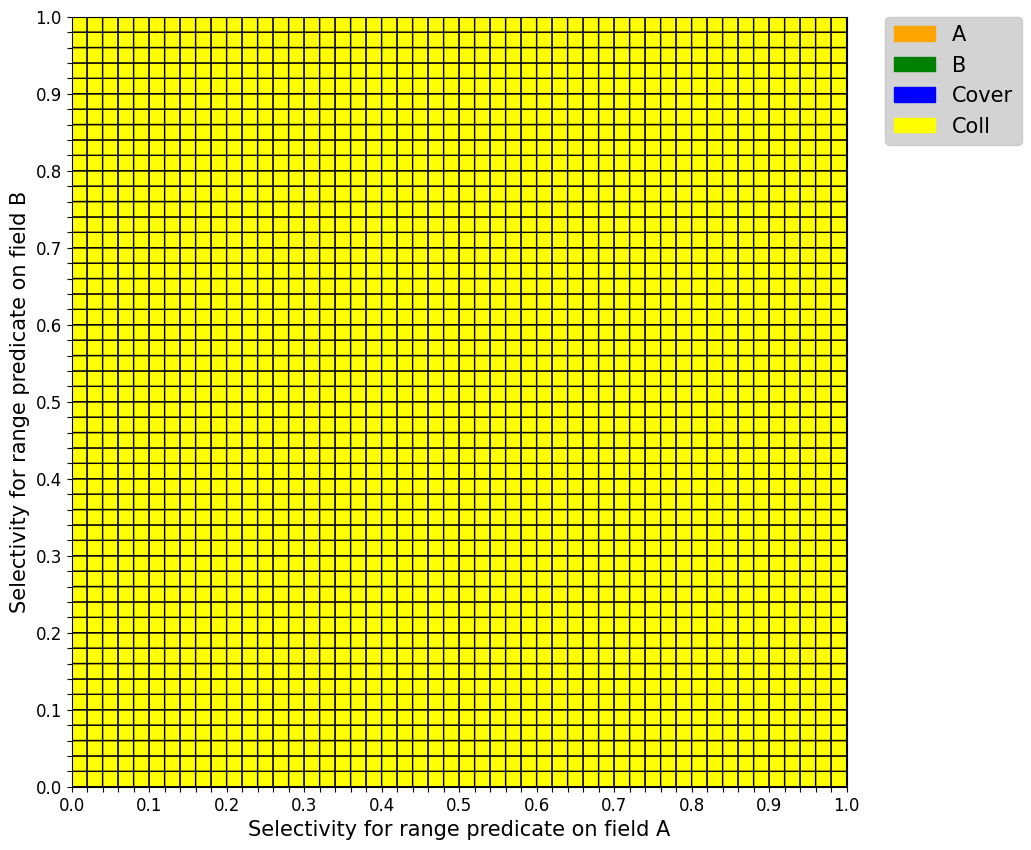
\includegraphics[width=0.6\linewidth]{images/results-without-covering-index/mongo-original/plan_coll_cached_mongo_choice.png}
    \caption{Plan C cached: MongoDB's chosen plans}
    \label{fig:c-cached-v0}
\end{figure}


\begin{figure}[htb]
    \centering
    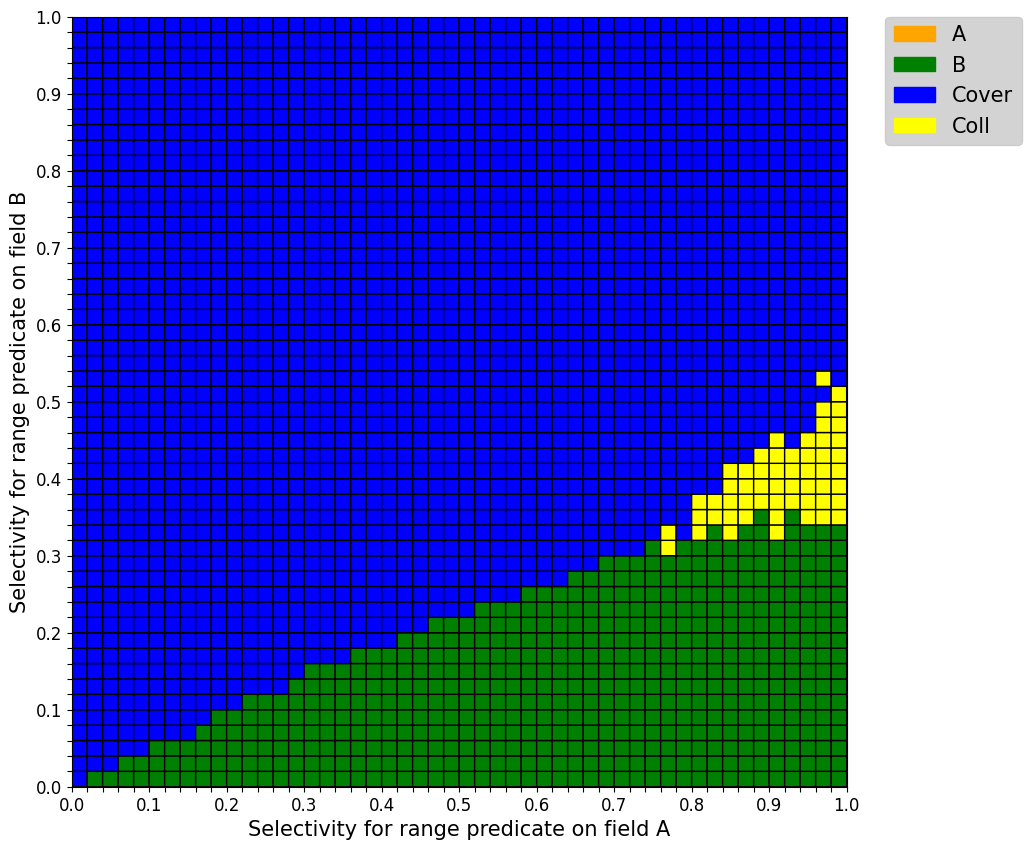
\includegraphics[width=0.6\linewidth]{images/results-without-covering-index/mongo-original/plan_coll_cached_practical_winner.png}
    \caption{Plan C cached: the optimal query plans}
    \label{fig:c-cached-optimal-v0}
\end{figure}


\begin{figure}[htb]
    \centering
    \includegraphics[width=0.5\linewidth]{images/results-without-covering-index/mongo-original/plan_coll_cached_summary_accuracy=47.48_overall_percentage_change=198.12.png}
    \caption{Plan C cached: MongoDB's chosen plans, accuracy = 47.48\%, impact factor = 198.12\%}
    \label{fig:c-cached-impact-v0}
\end{figure}


\clearpage